\chapter{概述}


\section{研究背景和意义}
无人机(UAV, Unmanned Aerial Vehicles)在最近十年中已经成为科技领域最吸引眼球的“关键词”。由于无人机自身具有成本低、机动性好、隐蔽能力强等特点,许多国家开展了基于无人机平台的各类研究。回顾历史,自1918年3月6日第一架现代无人机的出现距今已经近百年的历史,但在现实生活中,由于其安全性、可靠性等原因,无人机离我们的生活仍存在着一定的距离。特别是无人机在户外应用过程中,引导信息主要通过将GNSS信息与惯性导航信息相互融合得到。因此,在GNSS信号较弱或者发生中断的情况下,每年在世界各地均发生多起无人机坠毁事件,带来了巨大的人员和经济损失的同时,也限制了无人机的快速应用和发展。

在这些事故中,无人机操作员的失误导致的事故率高达60\%\cite{arrabito2010human}。在2004年的一份报告中指出\cite{williams2004summary},无人机的起飞和降落阶段过程中,人为因素的影响接近50\%。因此,研究精确可靠、自动化程度较高的着陆系统对无人机装备的战斗力生成至关重要,同时也是无人机通用技术发展的关键环节。下面针对自主起降技术的民用需求和军用需求展开说明。

\subsection{自主起降技术的民用需求}
近年来,随着我国经济的快速发展和人民生活收入水平的提高,越来越多的人选用民航作为出行手段,因此带来航班密度的显著增加。与此同时,气候原因与空气污染的综合作用导致航班晚点情况愈发严重。为研究气候原因导致飞机无法正常降落的情况,有文章\cite{BigDataLanding}通过分析2012年到2014年春运期间的民航数据(CADA, Civil Aviation Data Analysis)得出:影响航班准点率的雾、雪、霾天气所占比例为28.09\%;在千万级级别机场中,霾影响最严重的是郑州机场,占比例为29.21\%,其次是西安机场,所占比例为26.05\%;而在受雾影响的机场中,长沙机场占39.74\%,武汉机场占32.41\%,西安机场占32.07 \%。由此可见,在航班密度最大的春运期间,航班受天气影响导致延误的比例很大。

与人们直观的认知不同,航班是否能够安全降落,除飞机自身性能外,主要取决于目标机场的可见度情况,根据国际民航通用准则,飞机降落标准由低至高主要分为三类:CAT I类,其决断高度(DH, Decision Height)为$60\ m$、跑道视距(RVR, Runway Visual Range)为$550\ m$;CAT II类,DH为$30\ m$、RVR为$300\ m$;CAT III类,其DH和RVR均为$0\ m$要求,即为真正意义上的盲降。目前,国内除北京、浦东、成都、西安为II类机场外,多数机场为I类,而国内大多数航空公司只能执行I类标准,如果天气条件低于I类,航班就无法降落,只能选择备降或返航,影响航班正点率。因此,如果能够通过辅助设备,提高和拓展飞行员的可见度,则可以显著降低因为能见度原因导致的航班延误,从而提高民航的准点率。

在民用无人机领域,大量的无人机的回收依赖GNSS导航信息,加之没有配套的地面或舰载辅助引导设备,无人机的广泛应用受到了较大限制。

\subsection{自主起降技术的军事需求}
在军事领域,飞行器的自主起降需求则更为迫切。在有人机方面,随着2012年11月23日,歼-15战斗机首次在航母上成功实施阻拦着舰和滑跃起飞(如图\ref{fig:22_J15Landing_Big}所示),航母舰载机的引导降落问题再次引起世人关注。一般而言,为了保证舰载机正确返航和着舰,现代航母均配备有战术空中导航系统、空中交通管制系统和着舰引导系统。完整的着舰过程实质上是一场接力导航:当距离航母300公里时,归航舰载机由战术空中导航系统指挥引导;距离100公里时,由空管雷达接手;距离30公里时,再次由战术空中导航系统引导;距离10公里时,自动着舰系统开始引导;距离3公里时,进入舰上光学助降系统工作区域,最后据此着舰。

\begin{figure}[htb]
	\centering%
	\subfloat[X-47B着舰钩索的瞬间]{%
		\label{fig:01_X47B_Landing}
		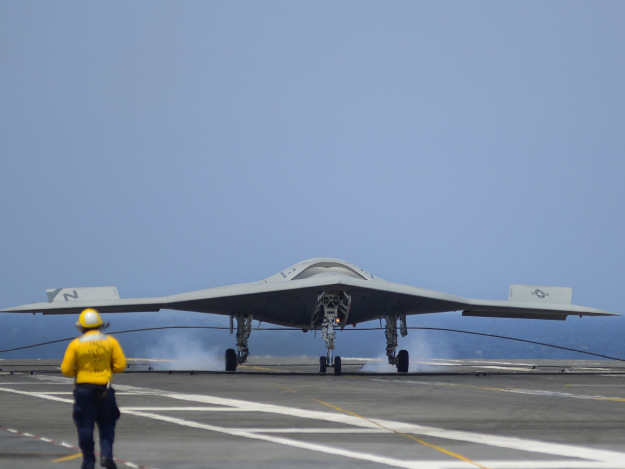
\includegraphics[height=5cm]{Figs/01_X47B_Landing.jpg}}\hspace{0.7em}%
	\subfloat[歼15着舰钩索的瞬间]{%
		\label{fig:22_J15Landing_Big}
		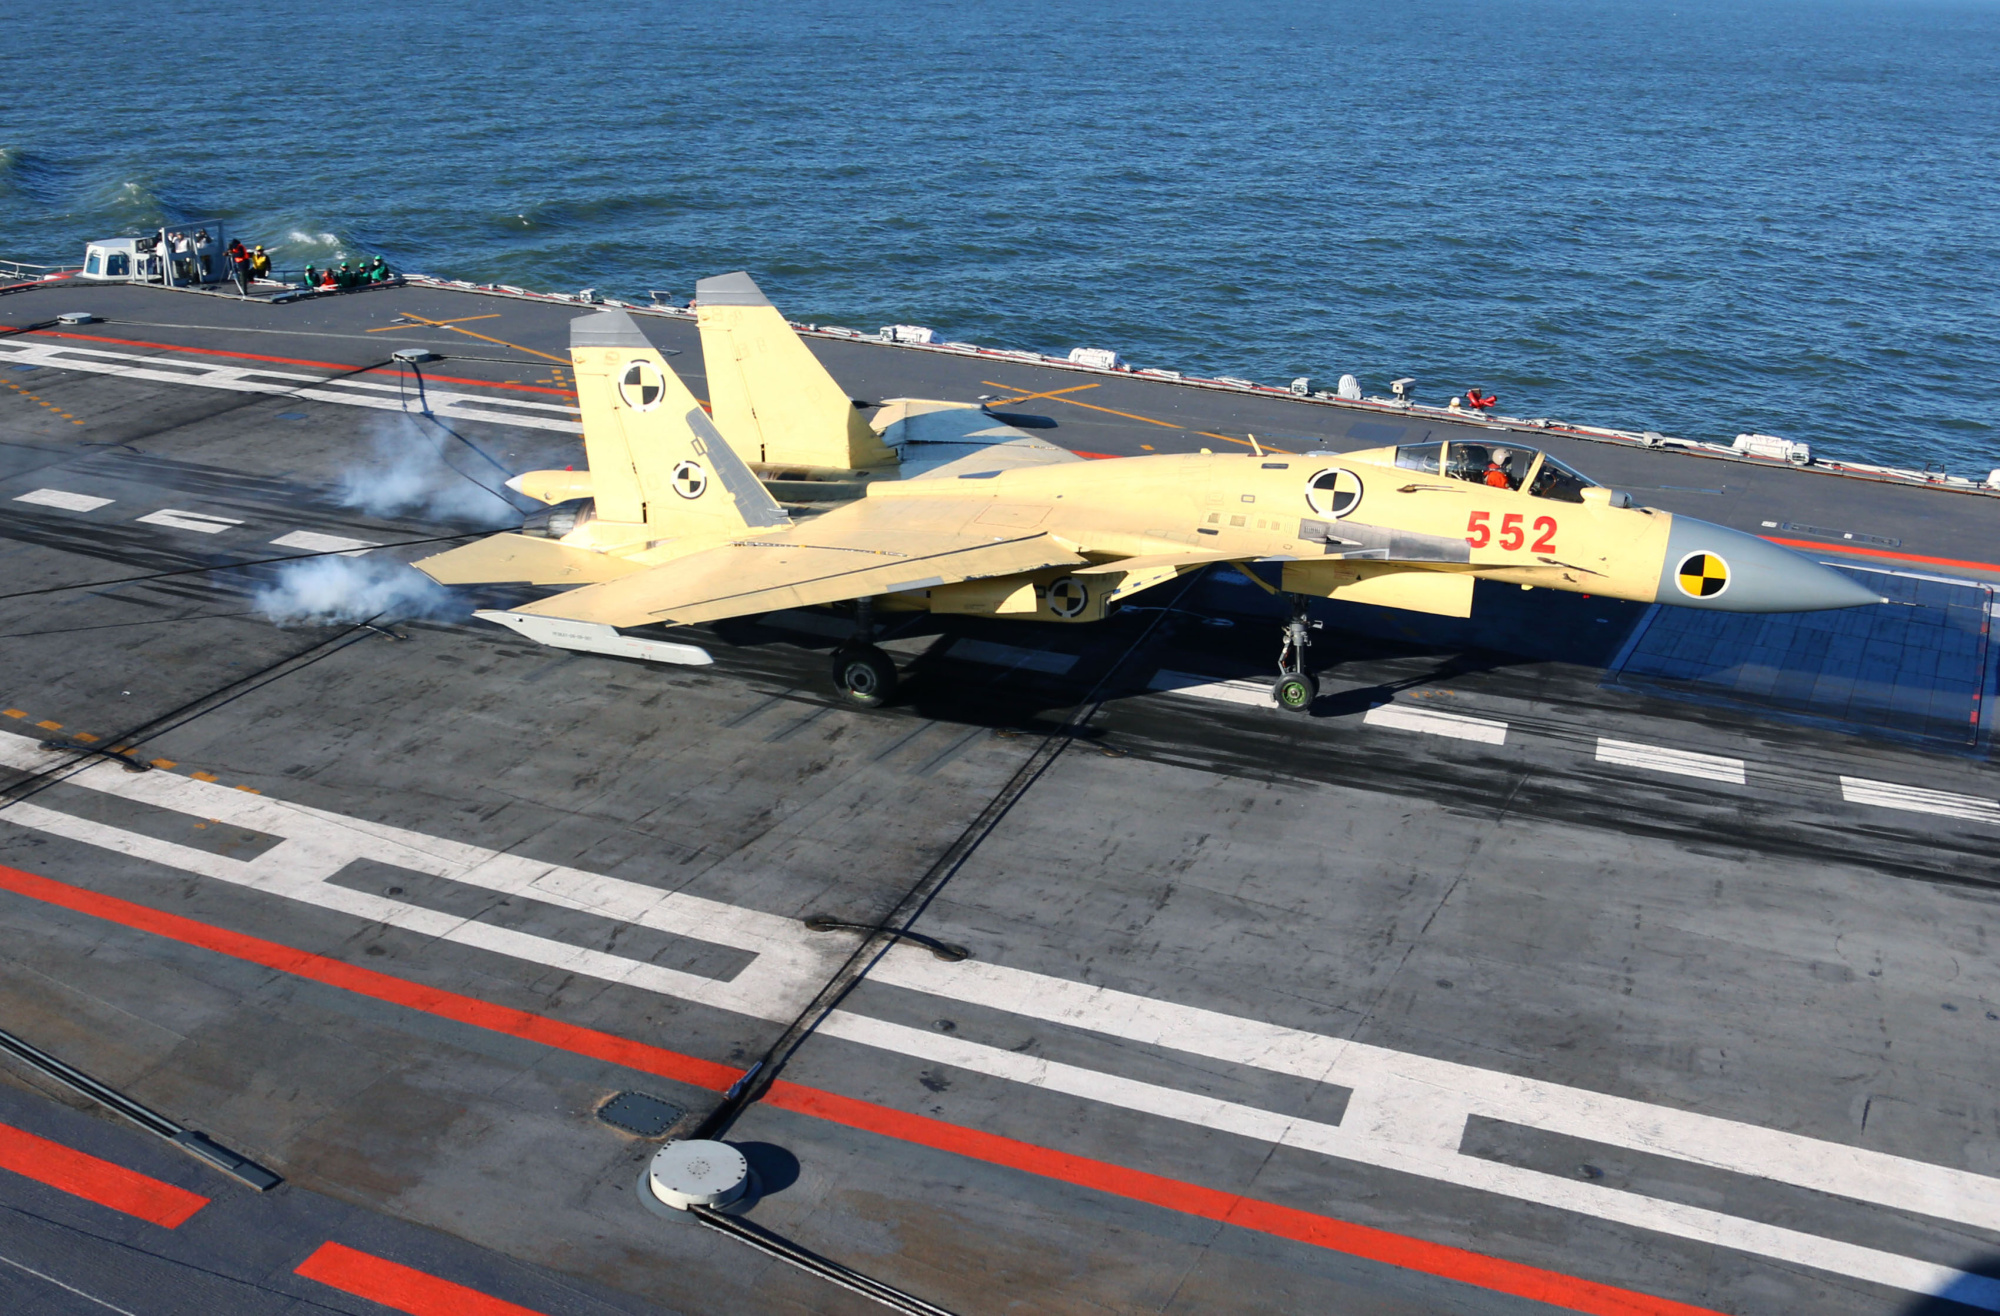
\includegraphics[height=5cm]{Figs/22_J15Landing_Big.jpg}}
	\caption{中美海军飞行器着舰瞬间}
	\label{fig:01_Landing}
\end{figure}

在舰载机降落过程中,飞行员除利用光学助降系统提供的信息进行修正外,航母舰舰载机着陆通常还依赖于人工辅助降落信息。在美航母上,通常由6人组成的着舰信号官(Landing Signal Officer,LSO)位于航母着舰区后部左舷,依靠视频监视系统所拍摄的实时图像及相应参数,通过无线电及灯光等多种手段对舰载机飞行员发出相应着舰指令(如图\ref{fig:20_LSO_USA}所示)。这6人分工和人员配置:(1)担当舰载机着舰引导操作的LSO;(2)利用飞行员助降视频(HUD)显控台引导飞机进场着舰顺序的助理LSO;(3)记录着舰成绩/等级的见习LSO;(4)担任舰内联络的下士联络员;(5)舰载机着舰前尾钩、起落架、襟翼状态的观察员;(6)负责监察着舰引导小组工作的负责人。而在公开的资料中,我国的有人机着舰也采用了类似LSO的人工辅助引导手段,其工作状态如图\ref{fig:21_LSO_China}所示。

\begin{figure}[htb]
	\centering%
	\subfloat[我国“辽宁号”航母上的LSO]{%
		\label{fig:21_LSO_China}
		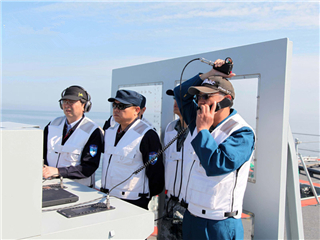
\includegraphics[height=4cm]{Figs/21_LSO_China.jpg}}\hspace{4em}%
	\subfloat[美军航母上的LSO]{%
		\label{fig:20_LSO_USA}
		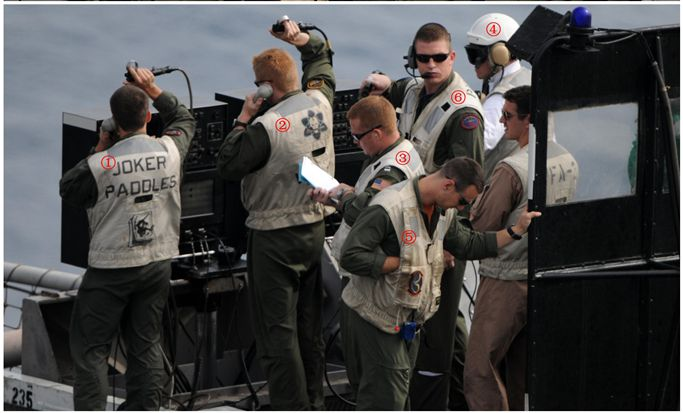
\includegraphics[height=4cm]{Figs/20_LSO_USA.jpg}}
	\caption{中美两国海军LSO工作图}
	\label{fig:21_LSO}
\end{figure}

无人机方面,在降落阶段无人机往往变成了“有人机”,一般会有多个人员进行操控和监视,以免出现差错。所以,本来希望减少人员工作负担的无人机,在降落阶段却往往成为让人担心的“微型炸弹”。为解决无人机的自主起降问题,早在2007年,美国诺斯鲁普·格鲁曼公司开始基于X-47B无人机和美国海军“无人作战航空系统-验证机”(UCAS-D)项目,开发和验证一种自主起飞/拦阻着舰型无人作战飞机。项目合同规定,诺格公司需要研制两架X-47B验证机,完成在航母上自主起降能力的验证,并在完成与航母一体化验证试验后,验证空中自主加油能力。如图\ref{fig:14_LandingAreaX47B2}所示,美国为开展相关研究,在Patuxent River试验基地展开岸基测试,并绘制了模拟甲板起降范围的模拟跑道(如图\ref{fig:10_LandingAreaX47B1}黄色箭头所示),这些细节体现了美国军方对这项技术的重视程度。
\begin{figure}[htb]
	\centering%
	\subfloat[位于海岸边的美军Patuxent River试验基地卫星图片]{%
		\label{fig:14_LandingAreaX47B2}
		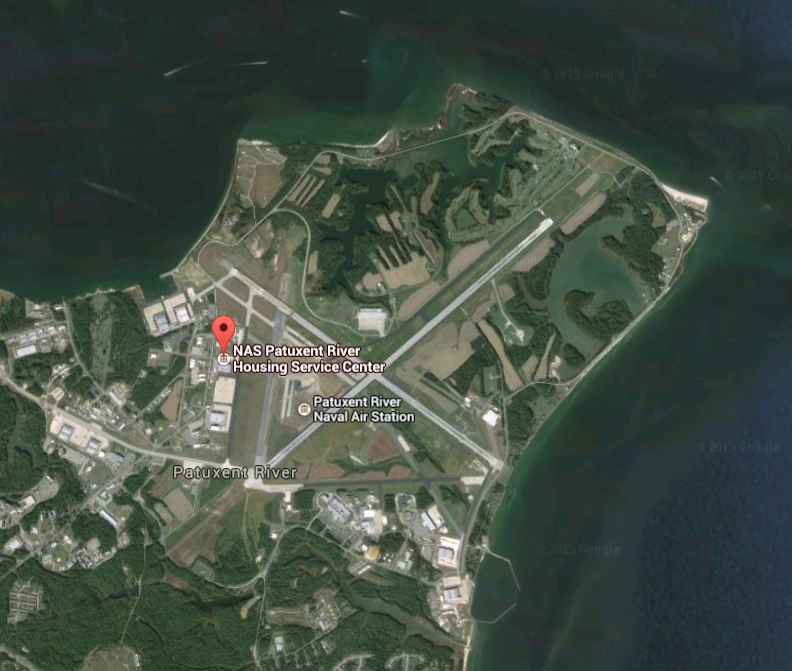
\includegraphics[height=6cm]{Figs/14_LandingAreaX47B2.jpg}}\hspace{0.7em}%
	\subfloat[黄色箭头所指为模拟航母甲板区域的专用跑道]{%
		\label{fig:10_LandingAreaX47B1}
		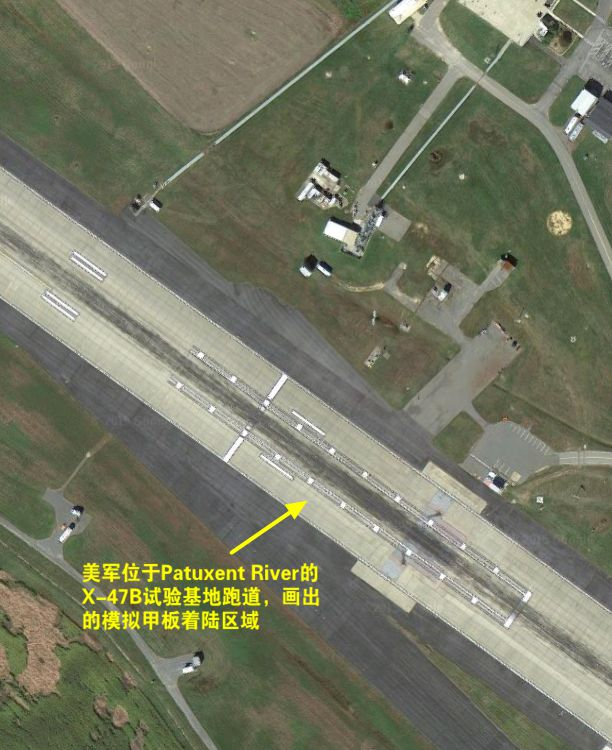
\includegraphics[height=6cm]{Figs/10_LandingAreaX47B1_1.jpg}}
	\caption{美军Patuxent River试验基地}
	\label{fig:14_LandingAreaX47B}
\end{figure}

在沉寂消息多年后,2013年7月,X-47B完成举世瞩目的首次航母自主降落,如图\ref{fig:01_X47B_Landing}所示)。根据公开资料显示\cite{X_47B},X-47B总共完成37次接触甲板测试(Deck Touchdown Test)和30次复飞(Touch-and-go)测试。在2014年3月,由于X-47B及其配套系统完成了人类历史上首次无人飞行器在航空母舰的全自主测试,“X-47B技术团队”获得美国航空协会最重要的“罗伯特·科利尔奖(Robert J. Collier Trophy)”\cite{X_47B_Award}。值得关注的是,该奖项曾经颁奖给诸多美国军用项目,如“全球鹰”无人机系统、“大黄蜂”战机系统、B2轰炸机系统等,由此可见X-47B及其配套系统在理论和工程上所具有的重要意义。此外,在各类报道中也特别提到:该系统精确的导航系统满足了飞行器降落在运动中的航母甲板上,具有里程碑意义\cite{X_47B_Report}。2014年8月,X47-B开展进一步测试,在完成与F/A-18F联合飞行验证后,在90秒内完成自主着舰、折叠机翼、撤出着舰区等一些列动作。其中,4次拦阻着陆,9次复飞再着陆。由于其优秀的控制性能,同月,美国海军计划利用X-47B开展空中自主加油的验证。X-47B的降落除机载传感器外,根据公开资料判断,舰载的JPALS或类似的雷达系统应当提供了辅助信息,如图\ref{fig:X47B_LandingOptical}所示。

\begin{figure}[htb]
	\centering%
	\subfloat[X-47B公布的视频中,跑道一侧的疑似毫米波雷达引导系统]{%
		\label{fig:09_X47BwithRadarGround}
		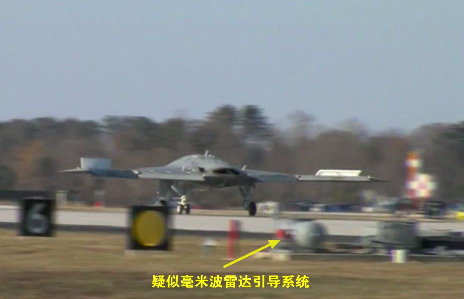
\includegraphics[height=5.2cm]{Figs/09_X47BwithRadarGround.pdf}}\hspace{1em}%
	\subfloat[X-47B公布的视频中,位于舰岛的疑似毫米波雷达引导系统]{%
		\label{fig:02_X47B_LanidngwithRadar1}
		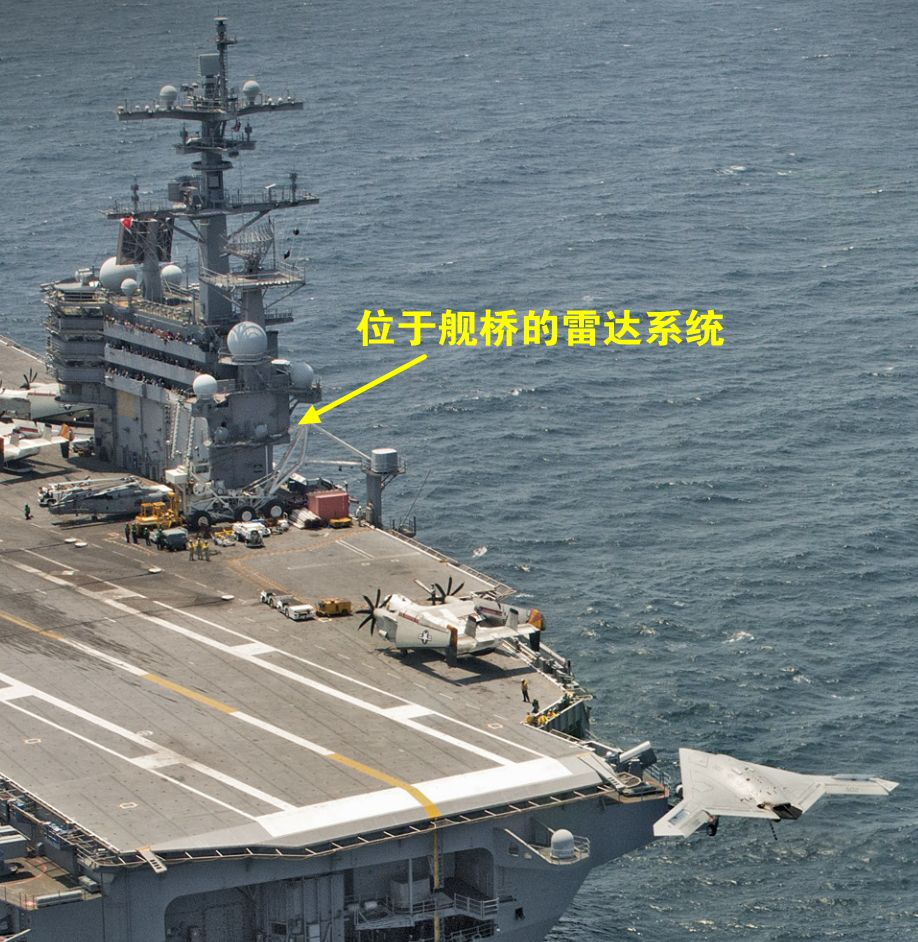
\includegraphics[height=5.2cm]{Figs/02_X47B_LanidngwithRadar1.jpg}}
	\caption{X-47B疑似使用的引导系统}
	\label{fig:X47B_LandingOptical}
\end{figure}



除X-47B这一机型之外,在2014年出版的《2030年的武器装备》\cite{2030equipment}一书中提到,作为美军太空机动飞行器(SMV)的验证机型X-37B轨道飞行器(OTV, Orbital Test Vehicle),其在返回过程中,运用航空器的导航与指导技术,采用惯性导航和GPS的组合式导航方式,在接近跑道前,以20°的下滑角,350 km/h的速度进场,其降落过程和姿态与X-47B相似(如图\ref{fig:31_X37B_Landing}所示)。根据公开资料显示,X-37B的自主再入和着陆系统采用了惯性导航和GPS的组合式导航。截至到2014年10月17日,X-37B已经完成三次飞行试验,其再入与着陆技术得到波音公司和美国军方的认可。此外,根据2015年2月23日的公开报道,X-37B轨道测试飞行器团队(X-37B Orbital Test Vehicle Team)荣获2015年美国AIAA颁发的年度最高奖项————杰出贡献奖(Award for Excellent)\cite{X_37B}。在颁奖的公告中特别提到,自主降落技术是X-37B的主要关键技术之一。

\begin{figure}[htb]
	\centering%
	\subfloat[X-37B降落沿跑道方向正视图]{%
		\label{fig:31_X37B_Landing1}
		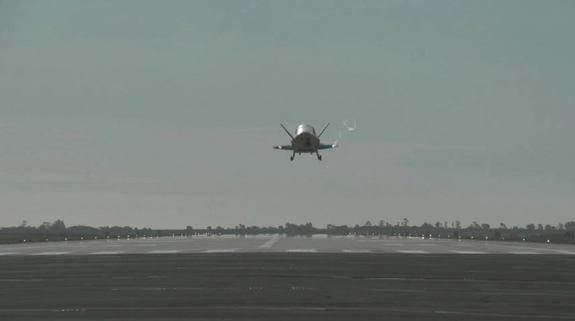
\includegraphics[height=4cm]{Figs/31_X37B_Landing1.jpg}}\hspace{0.7em}%
	\subfloat[X-37B降落侧视图]{%
		\label{fig:32_X37B_Landing2}
		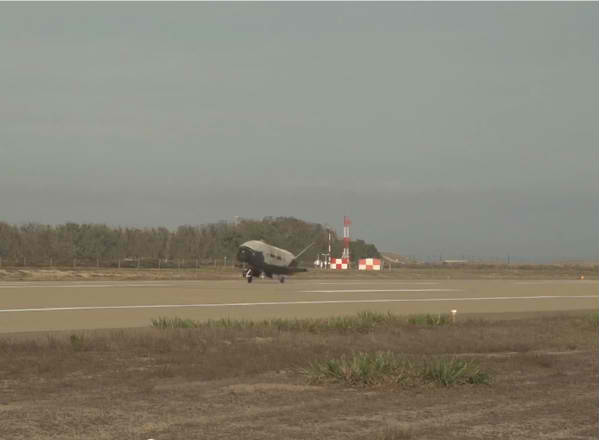
\includegraphics[height=4cm]{Figs/32_X37B_Landing2.jpg}}
	\caption{X-37B完成自主降落}
	\label{fig:31_X37B_Landing}
\end{figure}

综上所述,无人机自主起降技术,特别是舰载无人机自主起降技术是无人机广泛使用的基础和关键。能够在舰载环境,完成无人机的回收工作,具有很大的现实意义。


\section{军事和工业领域的引导降落系统}
\subsection{普通飞行器引导降落系统}
\subsubsection{仪表着陆系统}
在航空业发展初期,仪表着陆系统(ILS, Instrument Landing System)作为飞行器的主要着陆手段。该系统于1919年通过美国国家标准局的试验,并在二次大战期间得到广泛应用。1949年,国际民航组织规定仪表着陆系统作为着陆系统的国际标准。该系统主要由地面站和机载设备组成,主要通过机载接收机解算由地面航向信标和下滑信标独立产生的水平和交叉方向波束(波束频率不同),得到飞机的位置信息,即方位角、仰角和距离。该系统的示意图如图\ref{fig:07_ILS}所示。同时,民航组织根据需要,对不同气象条件下的进场标注进行了明确规定。其中,CAT I级别的高度主要通过气压计进行判读,CAT II和CAT III主要通过雷达高度计(Radio Altimeter)进行判读,不同级别的决断高度是飞行员做出是否复飞的基本准则。该系统的优点是具备较好的引导能力,可以为飞行员提供有效方位信息。但在当前电磁频谱环境复杂的机场附近,往往难以得到理想的引导控制精度,因此不能满足无人机系统的降落需求。该系统示意图如\ref{fig:07_ILS}所示。

\begin{figure}[htb]
	\centering%
	\subfloat[飞机在右偏,高度高于标准下滑曲线时的机载仪表显示]{%
		\label{fig:07_ILS1}
		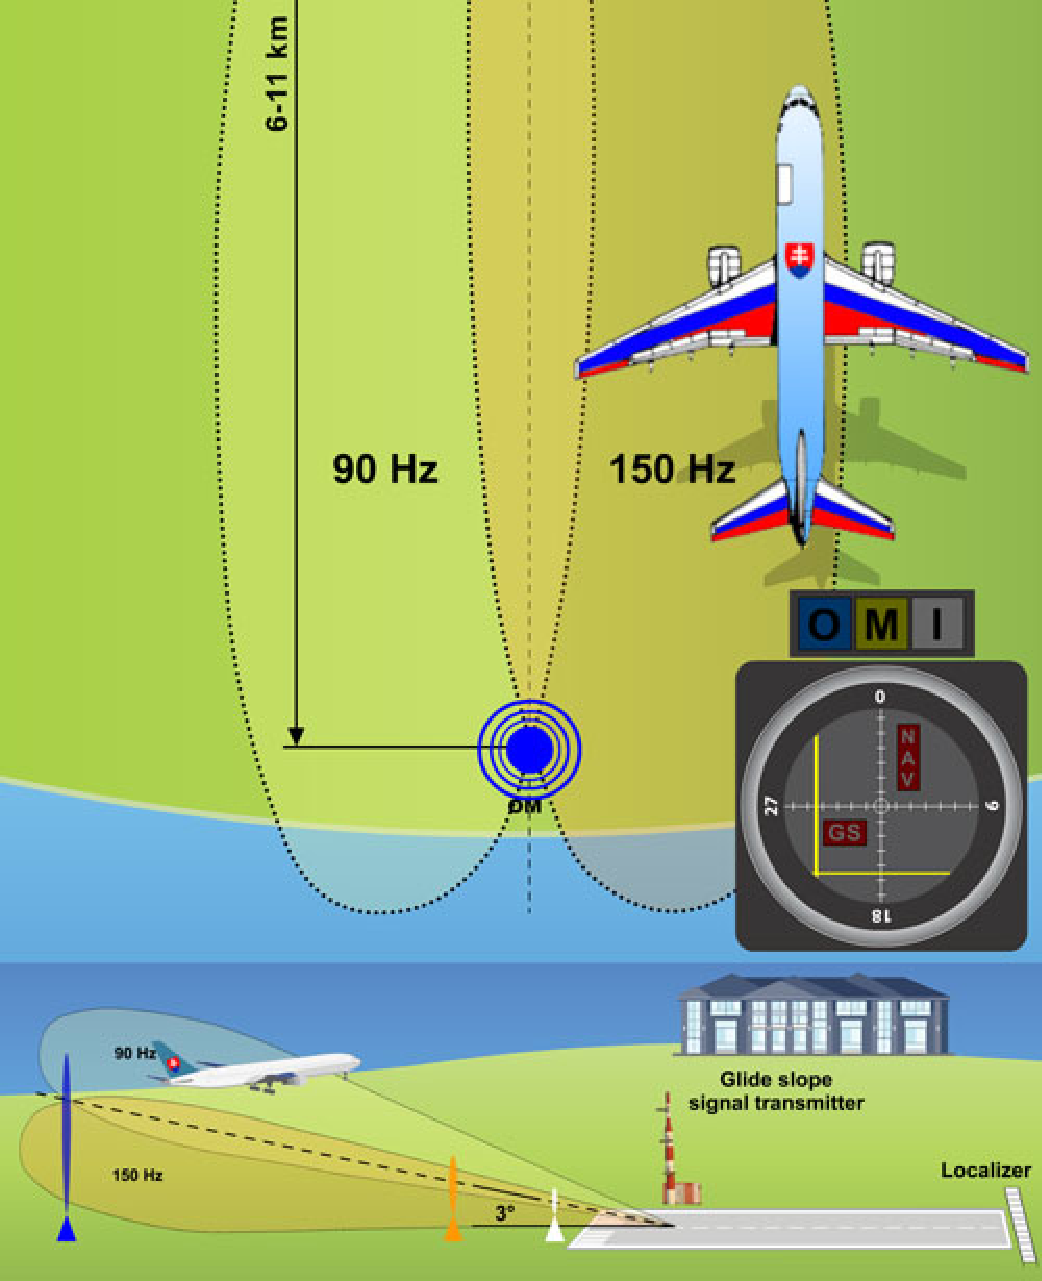
\includegraphics[height=7cm]{Figs/07_ILS1.pdf}}\hspace{4em}%
	\subfloat[飞机在左偏,高度低于标准下滑曲线时的机载仪表显示]{%
		\label{fig:08_ILS2}
		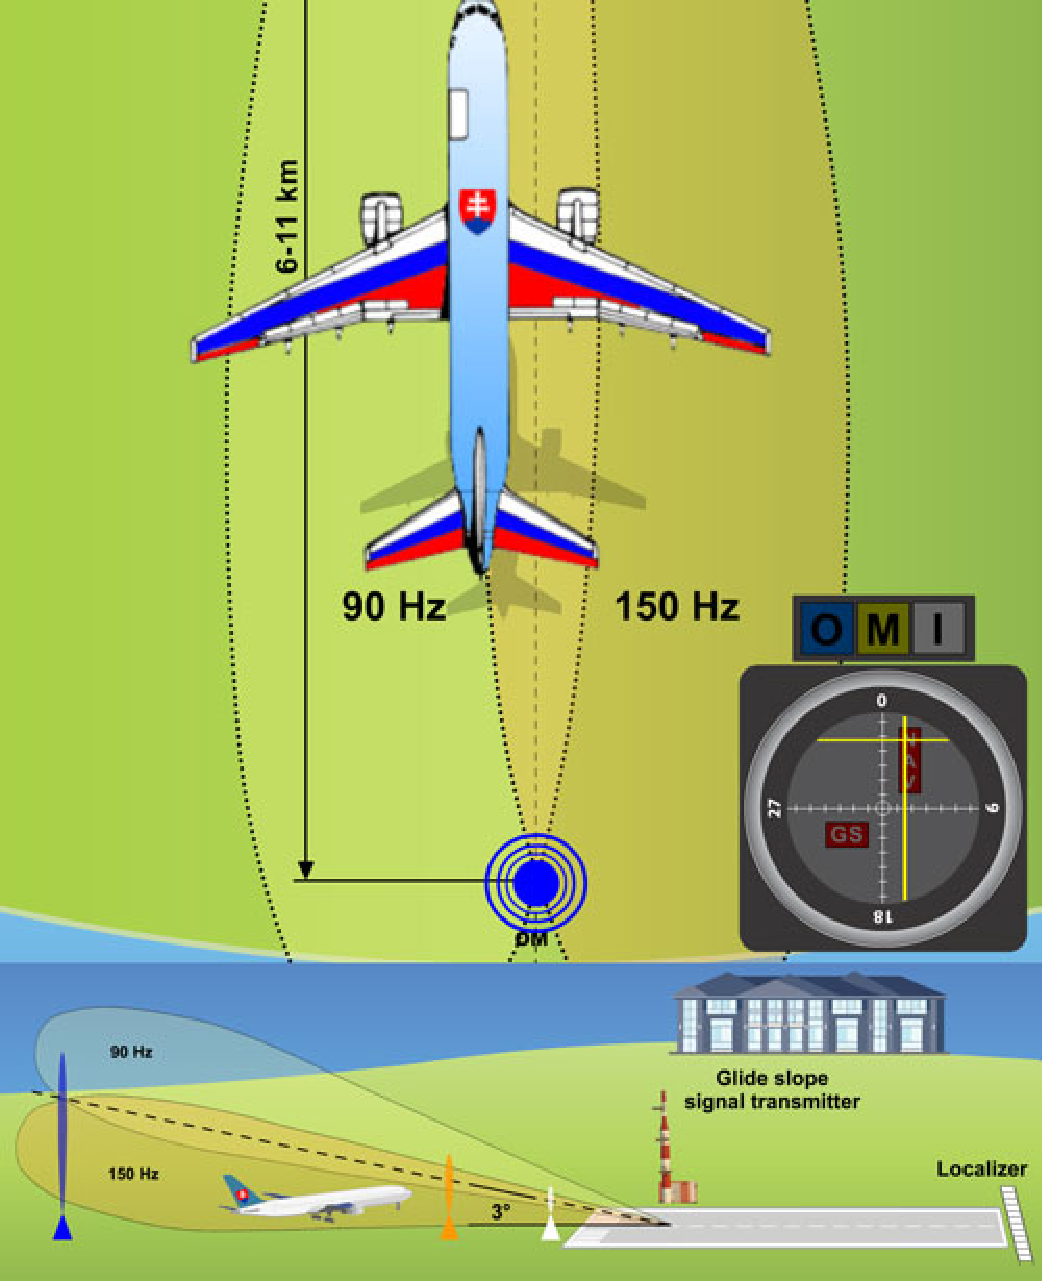
\includegraphics[height=7cm]{Figs/08_ILS2.pdf}}
	\caption{仪表着陆系统示意图}
	\label{fig:07_ILS}
\end{figure}

\subsubsection{雷达着陆系统}
随着二次大战对雷达在军事领域的广泛使用,美军在1943年研制了首套雷达着陆系统(GCA,Ground Control Approach),并于1946年拓展到民用领域。该系统通过地面引导雷达提供精确的位置信息,地面领航员根据雷达显示的下滑路径偏差与飞行员通话,进而操作飞机完成降落。随着技术发展,在雷达系统计算出下滑偏差后,可以根据飞机类型进行引导率计算,形成控制指令后反馈给飞机,协助飞行员或机载飞行系统完成下滑控制。这种方法也被称为“数据链+雷达”系统,至今仍然作为一种可靠的技术手段在航母和军用机场使用。

\subsubsection{微波着陆系统}
1978年,时间基准波束扫描技术(TRSB, Time Reference Scanning Beam)作为微波着陆技术的国际标准得到ICAO的认可。该系由地面方位台、仰角台、精密测距器和机载接收机组成。方位台和仰角台通过向空中发射扫描信号,机载接收机通过测量两次波束信号的时间间隔,得到飞机在空间的位置。但由于仪表着陆系统的广泛应用以及GNSS导航系统的迅猛发展,微波着陆技术的发展出现了一定的停滞。

\subsubsection{联合精密进近和着陆系统}
随着GPS和DGPS技术在美军的广泛应用,一套联合精密进近和着陆系统(JPALS)于2000年在地基完成测试实验。针对舰船本身和飞机都在运动,JPALS需采用双向的UHF数据链,将舰船测量到自身的GPS的位置,以及其摇摆、俯仰、偏航和向前运动的数据一并传给飞机,与此同时,飞机也将其GPS数据传回舰船。舰载的JPALS并不在意实际的位置误差,仅关注船和飞机偏离的量要相同,其着舰精度满足CAT III级别,纵向和横向精度控制在$1 \m$之内,能够完成航母着舰引导任务。在2005至2006年,JPALS开始替换现有的以雷达为基础的AN/SPN-46舰载精密进场着陆系统。这套系统还可用于舰上的空管,双向的数据链能使舰船以GPS跟踪、标注飞机方向。根据公布的合同要求,系统具备初始能力(IOC)时间为2019年,系统具备完全能力(FOC)时间为2030年。


\subsubsection{OPATS(Object Position and Tracking System)}
OPATS是瑞士RUAG宇航公司在1999年为瑞士空军开发研制的“目标定位跟踪系统”的简称,是一套基于激光技术的无人机自动着陆系统,用于瑞士空军的“巡逻兵”无人机。OPATS系统使用反射回来的激光信号对无人机进行跟踪,对目标无人机的动态位置进行连续测量跟踪,提供无人机在着陆阶段的可靠位置信息,并将高速更新的数据传输到地面站进行处,如图\ref{fig:15_OPTAS}所示。自1999年以来,RUAG已向全球范围内的众多用户交付了超过100套的OPATS系统。该系统的目标检测范围为35米至4000米,精度控制在1.5米。

\begin{figure}[htb]
	\centering%
	\subfloat[OPATS引导降落系统外场配置图]{%
		\label{fig:15_OPTAS1}
		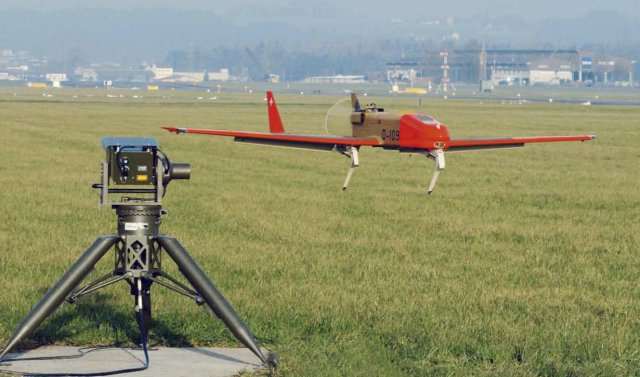
\includegraphics[height=4cm]{Figs/15_OPTAS1.jpg}}\hspace{4em}%
	\subfloat[OPATS引导降落系统框图]{%
		\label{fig:16_OPATS2}
		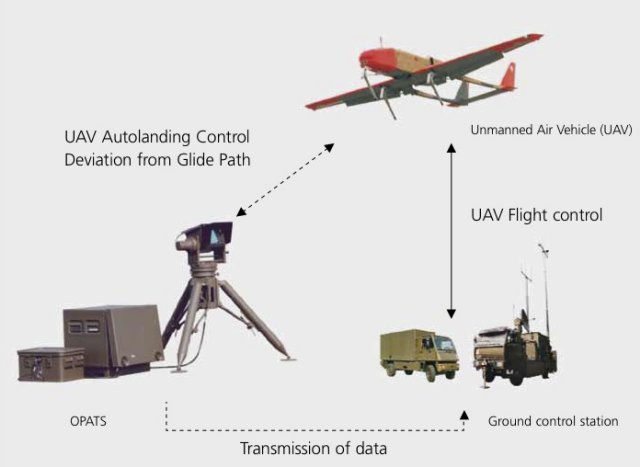
\includegraphics[height=4cm]{Figs/16_OPATS2.jpg}}
	\caption{OPTAS系统介绍}
	\label{fig:15_OPTAS}
\end{figure}


\subsubsection{光学引导系统}
光学助降系统主要依赖于“菲涅尔透镜”(Fresnel Lens)提供给飞行员相应的下滑曲线信息,以便飞行员操作飞机,即该引导系统是人在回路的引导方式。菲涅尔透镜有较好的聚焦性能,在同等焦距上由于传统球面透镜。由助降灯组和稳定平台组成,核心是位于中央的菲涅尔透镜和位于透镜两侧的水平基准灯。	舰载用的菲涅尔透镜系统(FLOLS, Fresenel Lens Optical Landing System)在传统的菲涅尔透镜基础上,将助降灯组与稳定平台结合。稳定平台的惯性系统可以检测舰船运动,使得射出的光束不受航母沉降摇摆的影响。在飞机进行着舰训练时,这套灯光组会释放出黄色、红色和橙色三种不同色彩光的下滑坡面,并以这三种光来界定高低位置。黄色光是高的下滑坡面,红色光是低的下滑坡面,橙色光是正确的下滑坡面。飞行员根据光所标定的位置在橙色光区域内下滑,就可以正确安全地着舰。


\subsubsection{基于UCARS的自主回收}
无人机通用自动回收系统(UAS Common Automatic Recovery System,UCARS)-V2系统(如图\ref{fig:29_UCARS})由内华达山脉公司(SNC)设计,为MQ-8B和MQ-8C火力侦察兵旋翼无人机的自主着陆提供引导控制。该系统是SNC的AN/UPN-51(V)无人机通用自动回收系统(UCARS)的改进型,并根据美军需求,拓展到其他型号的无人机引导降落,例如美国海军陆战队使用的先锋无人机。

该系统的主要传感器是毫米波雷达,该传感器也是军事和工业领域在引导无人机降落过程中使用最多的传感器质之一。毫米波雷达比普通的微波雷达体积更小,同时还具备波束窄和抗干扰能力强的特性;相比于红外传感器,毫米波雷达对于雨雾天气和灰尘的穿透性更强。UCARS系统主要由机载应答系统和舰载跟踪系统组成。跟踪传感器可以检测并计算无人机相对于期望降落点的位置信息,并向无人机提供降落平台的位置和运动状态数据,便于机载系统的导航和控制。目前UVARS系统有V2改进版,该版本使得无人机具备自主降落能力,减少了无人机飞行员的干预。此外,它还具备船舶运动稳定设备,以满足不同海况下的运行需求,该系统的引导控制精度在2.5厘米左右。系统的地基和舰载配置情况如图\ref{fig:29_UCARS}所示。 

\begin{figure}[htb]
	\centering%
	\subfloat[UCARS引导庞巴迪CL-227降落]{%
		\label{fig:29_UCARS1}
		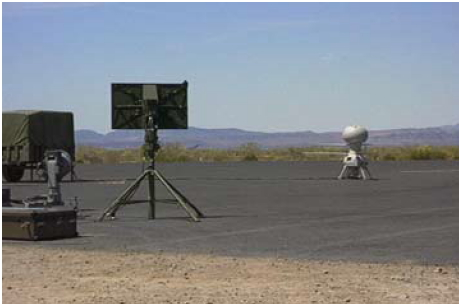
\includegraphics[height=4cm]{Figs/29_UCARS1.jpg}}\hspace{1em}%
	\subfloat[UCARS引导MQ-8B降落]{%
		\label{fig:30_UCARS2}
		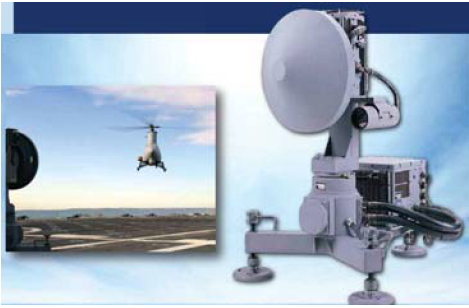
\includegraphics[height=4cm]{Figs/30_UCARS2.jpg}}
	\caption{无人机通用自动回收系统(UCARS)}
	\label{fig:29_UCARS}
\end{figure}

\subsubsection{无人机甲板起降引导系统}
法国DCNS公司开发的无人机直升机甲板起降引导系统(SADA\footnote{此处为法语缩写,Systèmed’Appontage et de Décollage Automatique})\cite{DCNS}使用红外传感器精确跟踪无人机,同时发出飞行指令调整航线直到确保无人机的“鱼叉”式着陆装置对准降落格栅的中心。2008年10,SADA成功将一架奥地利西贝尔公司研制的“坎姆考普特”(Camcopter)S-100无人直升机以自主模式降落在一艘正在地中海航行的法国海军驱逐舰“蒙特卡姆”号(Montcalm)上。该系统的引导控制精度约$30\ cm$。

\begin{figure}[!tb]   
	\centering	
	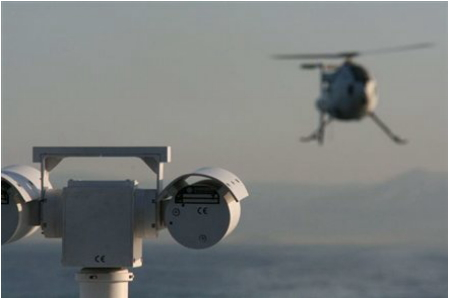
\includegraphics[width=0.5\textwidth]{Figs/24_SADA_Landing.jpg}
	\caption{SADA系统引导无人直升机着舰 }
	\label{fig:24_SADA_Landing}
\end{figure}


\subsubsection{基于D2AD自动甲板起降系统}
2011年,法国DCNS公司和Thales 公司完成无人机直升机在甲板自主降落(D2AD\footnote{此处为法语缩写,Démonstration d'un système d'appontage et d'atterrissage pour drones})的测试。此次海试使用法国海军“拉斐尔”级护卫舰和一架波音H-6U“小鸟”旋翼无人机,实验标志着 D2AD项目为期 4 年的技术验证成果。D2AD系统包括“飞行”部分和“地面”部分,“飞行”部分是无人机的指引标,“地面”部分在飞行甲板使用传感器进行船体运动预报,是无人机的引导站(如图\ref{fig:25_D2AD})。D2AD不依赖于任何卫星定位系统,能够保证垂直起降无人机在舰船上的安全使用。

\begin{figure}[htb]
	\centering%
	\subfloat[D2AD自主甲板降落系统]{%
		\label{fig:25_D2AD_1}
		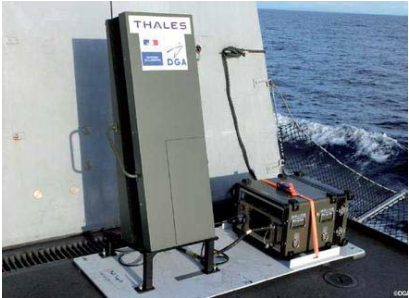
\includegraphics[height=4cm]{Figs/25_D2AD_1.jpg}}\hspace{0.1em}%
	\subfloat[H-6U“小鸟”旋翼无人机]{%
		\label{fig:26_D2AD_2}
		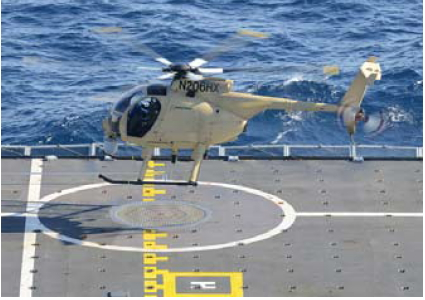
\includegraphics[height=4cm]{Figs/26_D2AD_2.jpg}}\hspace{0.1em}
	\subfloat[机载指引标]{%
		\label{fig:27_D2AD_3}
		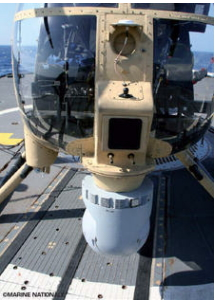
\includegraphics[height=4cm]{Figs/27_D2AD_3.jpg}}
	\caption{D2AD机载引导系统基本构成}
	\label{fig:25_D2AD}
\end{figure}

\subsubsection{基于DeckFinder的降落系统}
2013年6月,奥地利西贝尔电子设备公司的“坎姆考普特”S-100 无人直升机配装欧洲航宇防务集团(EADS)阿斯特里姆公司的“甲板发现者”(DeckFinder)区域定位系统,在一周的时间内完成了一系列旨在演示验证GPS干扰环境中无人机自动起飞与回收能力的飞行试验。“甲板发现者”系统\cite{Deckfinder}包括地面部分和机载部分,其中地面部分包括6台射频发射机,机载部分包括1台接收机。该系统的测距不依赖于GPS,可为航空器提供高精度的三维相对位置信息。根据公布的技术细节,该系统的工作范围约为$1.1\ km$,降落阶段精度优于$20\ cm$,工作频率不低于$15\ Hz$。
\begin{figure}[!tb]   
	\centering	
	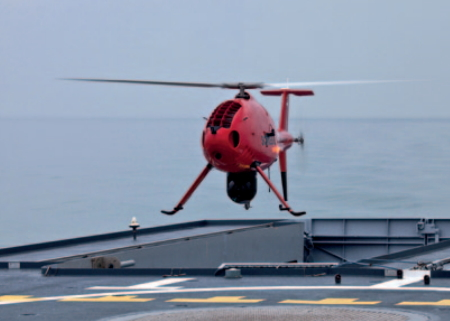
\includegraphics[width=0.5\textwidth]{Figs/28_Deckfinder.jpg}
	\caption{DeckFinder在GPS干扰环境下引导S-100无人机降落}
	\label{fig:28_Deckfinder}
\end{figure}

\subsubsection{基于JPALS的引导降落}
% X-47B
作为固定翼无人作战飞机,X-47B无人机面临着与其他无人机同样的难题:回收过程复杂。根据海军科技网站(Naval Technology)公布的消息\cite{X_47B_UCAS},X47-B的引导控制系统有较强的自主性,其导航系统主要由GPS和视觉系统组成。为提高智能化程度,X47-B还配备了光学系统、红外系统、SAR雷达(SAR, Synthetic Aperture Radar)、地面目标指示器(Ground mMving Tagret Indicator)和海面目标指示器(Maritime Moving Target Indicator)等设备。此外,在自主降落过程中,系统遵循预设的下降曲线对飞机进行引导和控制,操作员只是监视整个下降过程。虽然X-47B使用的具体引导降落方式没有公开,但通过公开视频和图像分析(如图\ref{fig:X47B_LandingOptical}所示),X-47B的自主着舰也应用了类似引导系统。

通过阅读相关资料并分析,该联合精确进场与着舰系统(JPALS)由处理、维修和监测系统,UHF数据链,惯性传感器和GPS传感器等组成,可以实现高可靠性和可用性。JPALS将与AN/TPX-42空中交通管制雷达、AN/SPN-46自动着舰系统、AN/SPN-41着舰辅助雷达、着舰信号官显示系统、改进型菲涅耳透镜光学着舰系统、航空数据管理和控制系统集成。2011年7月,F/A-18D“大黄蜂”战机在“艾森豪威尔”航空母舰上实现无人控制自主降落。

% ----- MQ-8B/C
2006年1月,MQ-8B完成了第一次在两栖登陆舰USS Nashville的舰载着陆,实验海域为Chesapeake Bay。2014年8月27日,MQ-8C“火力侦察兵”无人直升机在文图拉县海军基地完成着舰试验。

\subsection{无人机回收方式概述}
在X-47B无人机成功阻拦降落之前,世界各国在舰载无人机回收方面普遍采用的方法是:撞网回收、打捞回收和钩绳回收等。其中,撞网回收和钩绳回收对无人机回收控制精度提出更高要求,需要无人机自身或舰基系统具有较好的引导和控制能力。

\subsubsection{伞降回收}
伞降回收就是利用降落伞回收无人机。无人机从飞行状态到安全回收,整个过程自动完成,对操作人员要求较低。这种回收方式操作简单,是小型无人机回收的一种重要方式,适合对落点没有特殊要求的回收。采用轮式着陆的无人机也可使用伞降回收作为应急回收方案。采用水上伞降回收时,要考虑到无人机落入水中后对机身和内部设备的影响。

\subsubsection{撞网回收}
使用拦截网系统回收无人机是目前小型无人机较普遍采用的回收方式之一。无人机在降落阶段,通过降低高度和减小速度,撞向由弹性材料编制成的阻拦网。美国RQ-2“先锋”无人机和“银狐”无人机均采用
这类回收方式,如图\ref{fig:34_RQ2_Pioneer_Landing}所示。
\begin{figure}[!tb]   
	\centering	
	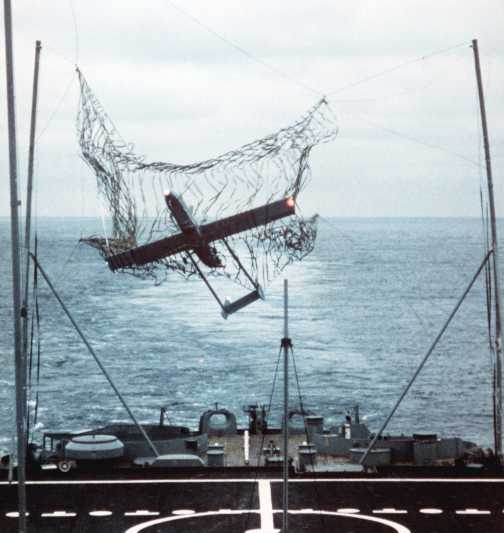
\includegraphics[width=0.4\textwidth]{Figs/34_RQ2_Pioneer_Landing.jpg}
	\caption{RQ-2在舰船完成撞网回收}
	\label{fig:34_RQ2_Pioneer_Landing}
\end{figure}

% Bat UAS
%翼展4.26 m、极长2.0 m、最大起飞重量159 kg、有效载荷34 kg。
%Shadow
%Poineer

\subsubsection{钩绳回收}
该回收方法使用垂直悬浮钢丝的天钩技术。钢丝可以自由的悬浮在吊杆上或者通过风筝把它升起,同时在无人机的翼尖上固定一个自锁的钩子。无人机进场时,径直地飞向钢丝,以便钢丝碰到其中一个机翼的前缘,然后滑向翼尖,通过钩子便可以把无人机锁住。由于航母的摆动幅度通常会限制为横摇2-3度,纵摇1-1.5度,而中小型船只稳定性要差得多,因此必须在横摇13度,纵摇5-6度的恶劣环境下,相比撞网回收,钩绳回收的引导控制需求更高,需要确保无人机在一米大小的回收窗口准确降落。

RQ-21A在2010年称为美国小型战术系统(Small Tactical Unmanned Aircraft System)项目的主力机型,该飞机具备陆基和海基起降能力,能够完成战术侦察、监视、目标指示(Reconnaissance, Surveillance and Target Acquisition,RSTA)功能,其模块化设计可快速替换不同传感器并完成部署。2014年7月,美国海军开始使用RQ-21A系统进行海上综合测试。该型无人机采用钩绳回收方式,如图\ref{fig:33_RQ21_Landing}所示。此外,“扫描鹰”无人机也采用此类方式回收,如图\ref{fig:35_Eagle_Scanner_Landing}所示。

\begin{figure}[htb]
	\centering%
	\subfloat[RQ-21在舰船回收]{%
		\label{fig:33_RQ21_Landing}
		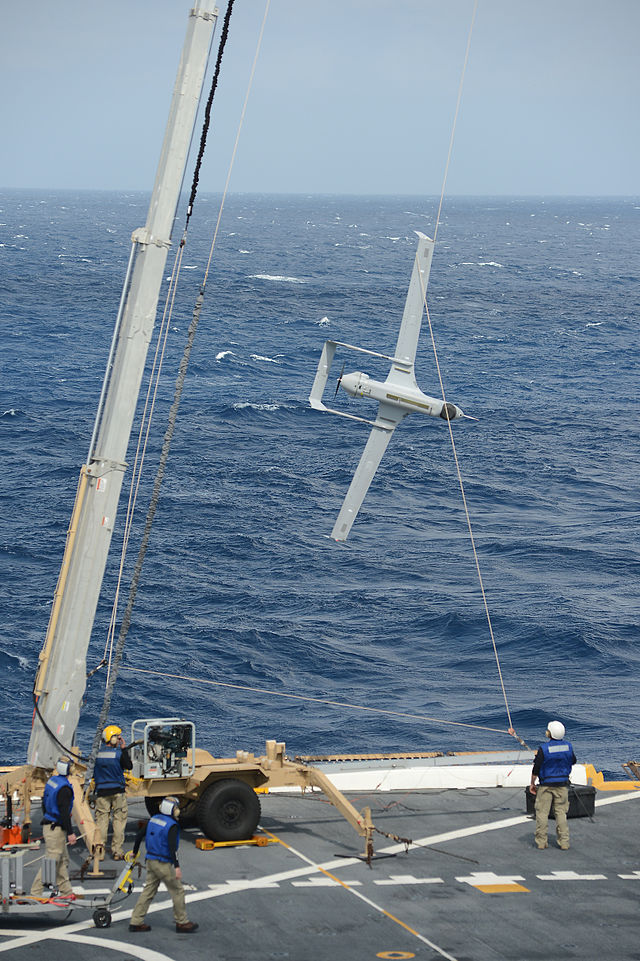
\includegraphics[height=6cm]{Figs/33_RQ21_Landing.jpg}}\hspace{0.1em}%
	\subfloat[“扫描鹰”无人机在舰船回收]{%
		\label{fig:35_Eagle_Scanner_Landing}
		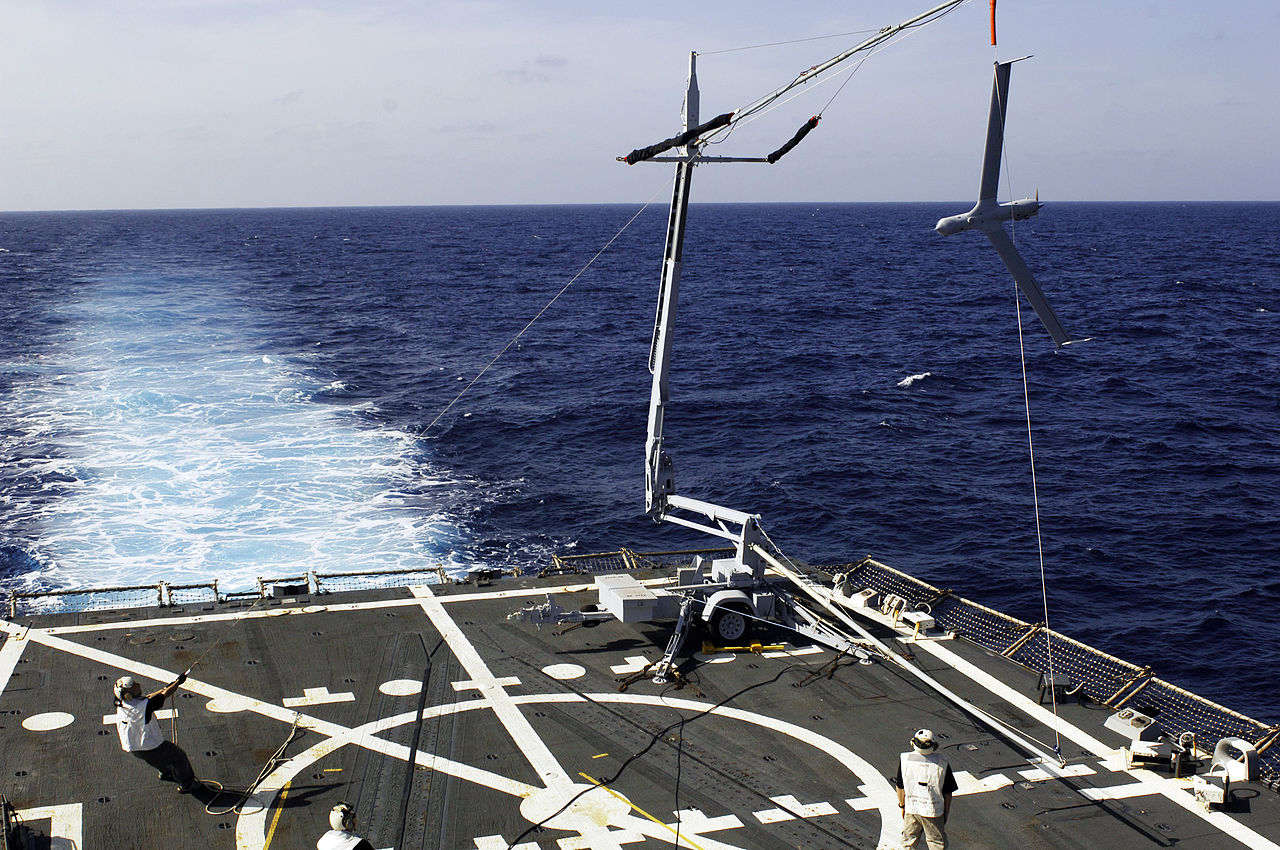
\includegraphics[height=6cm]{Figs/35_Eagle_Scanner_Landing.jpg}}\hspace{0.1em}
	\caption{采用钩绳回收方式的无人机}
	\label{fig:33_RQ21withScanner_Landing}
\end{figure}


\section{学术研究领域的无人机引导降落系统}
由于可见光摄像机成本低廉的特点,基于图像信息的无人机引导和控制在无人机实际应用中扮演十分重要的角色。例如,利用机载摄像机来完成感知规避任务\cite{mejias2010vision}、监视和跟踪任务\cite{campoy2009computer}\cite{mejias2006visual}、自主起飞和降落任务\cite{saripalli2002vision}、实时建图与定位任务(SLAM)\cite{weiss2011monocular}等。此外,通过图像信息对无人机自身位置和姿态进行估计也是今年来的研究重点和热点。比如在空中加油领域、无人机定点区域着陆等。2014年,针对视觉在无人机自主降落领域的研究现状,文章\cite{kong2014vision}系统总结了当前37个世界各地研究单位的工作,总结表格详见附录。本节只针部分内容进行概述。

\subsection{机载传感器引导降落系统} 

早在2003年,Shakernia\cite{shakernia2003vision}的博士论文中提出一种基于视觉的旋翼无人机(Yamaha R-50)的自主降落方案,该方案通过识别放置于六自由度运动平台上的合作标志完成自主降落(如图\ref{fig:chp01_06_shakernia_landing}所示)。其中,通过识别合作标志中的焦点,并使用Linear Two-view Motion Estimation, Non-linear Two-view Motion Estimation和Multi-view Planar Algorithm方法对飞机的位置和姿态进行估计。上述三种方法可以较好的解决特征点共面的飞机和位置姿态估计问题,通过仿真和户外试验,验证了系统的有效性和鲁棒性(位置偏差小于0.05米,角度偏差小于0.5°),但对于非合作目标的识别,不具备求解的通用性。

\begin{figure}[!tb]   
	\centering	
	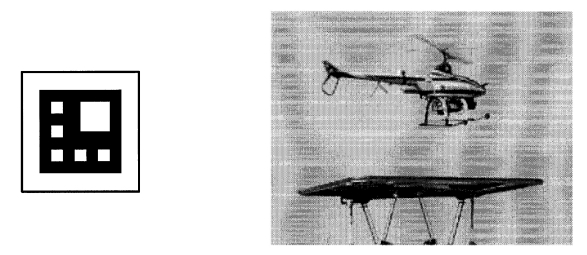
\includegraphics[width=\textwidth]{figs/chp01/chp01_06_shakernia_landing.pdf}
	\caption{基于合作标识的无人直升机自主降落系统\cite{shakernia2003vision}}
	\label{fig:chp01_06_shakernia_landing}
\end{figure}


2009年,朱建明\cite{Zhu_Master_2009}对传统“H”形合作目标进行改进将“H”形图标的上端开口封住,改进后的图标能够克服“H”形图标缺乏有方向性的缺点,在地标图案分割的基础上,采用基于灰度变化的角点检测方法,提取合作标志的特征点。

2010年之后,该领域的研究逐渐增多。韩国科学技术院(Korea Advanced Institute of Science and Technology,KAIST)提出一种应用于小型无人机上的视觉引导着陆系统通过视觉引导无人机飞行至安装在地面上的红色圆拱形安全气袋中\cite{huh2010vision},原理如图\ref{fig:chp01_05_korea_landing}所示。
\begin{figure}[!tb]   
	\centering	
	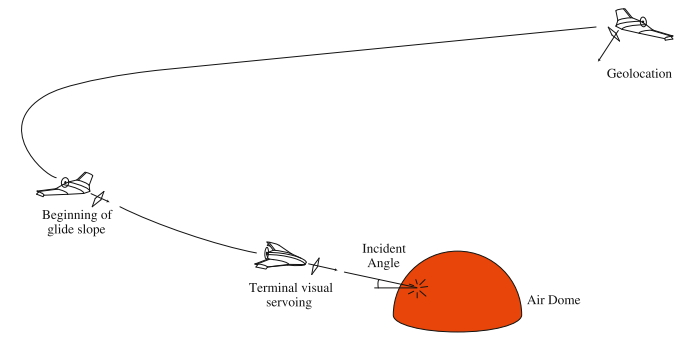
\includegraphics[width=\textwidth]{figs/chp01/chp01_05_korea_landing.pdf}
	\caption{基于红色标志物的无人机回收系统示意图\cite{huh2010vision}}
	\label{fig:chp01_05_korea_landing}
\end{figure}

李宇\cite{Li_Master_2012}设计了一种由6个圆心已标识出来的红色圆圈组成的合作标志,通过基于仿射不变矩和SVM分类器实现着陆地标的识别,如图\ref{fig:chp01_04_six_circle_landing_pattern}所示。
\begin{figure}[!tb]   
	\centering	
	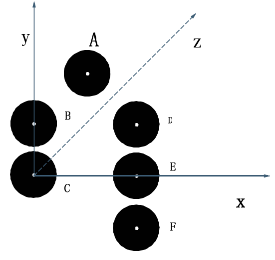
\includegraphics[width=0.4\textwidth]{figs/chp01/chp01_04_six_circle_landing_pattern.pdf}
	\caption{六个圆形合作标识\cite{Li_Master_2012}}
	\label{fig:chp01_04_six_circle_landing_pattern}
\end{figure}

H. Jin Kim等人\cite{kim2013fully},针对小型固定翼无人机一种基于机载视觉的撞网回收系统。该系统采用颜色分割和形态学等图像处理算法,通过机载摄像头对无人机回收网进行检测和识别;通过几何位置分析,判断无人机当前的方位信息,设计无人机引导率和控制率;地面控制系统可以向无人机发送控制命令并监测无人机的飞行状态。

德国宇航局在2015至2016年进行了HALE(High Altitude Long Endurance) UAV在运动汽车顶部回收的实验测试,该型号无人机的翼展为$3.3\ m$,最大起飞重量为$21.5\ kg$。该无人机在距离地面车辆$300\ m$左右的距离捕获地面移动车辆,随后地面移动车辆加速至合适的速度,满足无人机的回收需要。在回收过程中,无人机的引导方式主要通过机载摄像机对汽车顶部的合作标识(二维码)进行识别,进而实现相对位置的解算,完成自主降落\cite{Muskardin2016}。由于合作标识的尺寸和机载相机视场角的约束,无人机检测到地面目标点的距离较短,系统有效工作范围较小。
\begin{figure}[htb]
	\centering%
	\subfloat[无人机在回收末状态时,与汽车的速度保持相同]{%
		\label{fig:07_ILS1}
		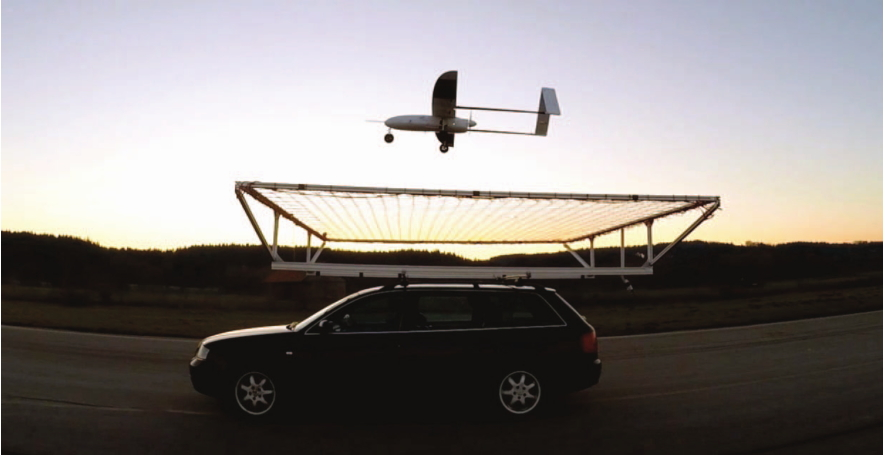
\includegraphics[height=3.5cm]{figs/chp01/chp01_01_DLR_Landing.pdf}}\hspace{0em}%
	\subfloat[机载传感器通过识别车顶的合作标识,实现相对位置的解算]{%
		\label{fig:08_ILS2}
		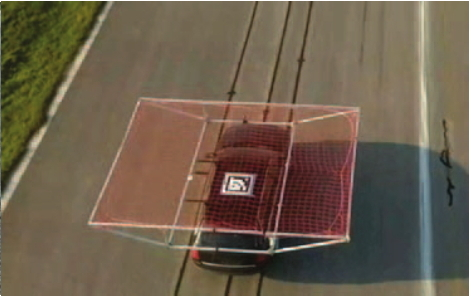
\includegraphics[height=3.5cm]{figs/chp01/chp01_02_DLR_Landing_with_tag.pdf}}
	\caption{德国宇航局车载无人机回收试验图\cite{Muskardin2016}}
	\label{fig:07_ILS}
\end{figure}

2016年5月,卡内基梅隆大学的研究者发布了最新无人直升机降落在海面移动平台\cite{Grocholsky2016}的工作。无人机上装载了长波红外传感器,该传感器适应雨雾天气,最远探测海面移动平台的距离为1.2海里(约2.22公里)。无人机从500米开始,对海面移动平台进行位置估计,并逐渐靠近该平台。在距离195米左右时,机载可见光传感器可以识别位于降落平台的合作标识,并具备对该平台姿态进一步估计的能力,其识别效果如图\ref{fig:chp01_03_CMU_Sea_Landing}所示。在最后50米的距离,激光传感器通过对甲板的三维空间扫描,实现厘米级的位置解算精度。

\begin{figure}[htb]   
	\centering
	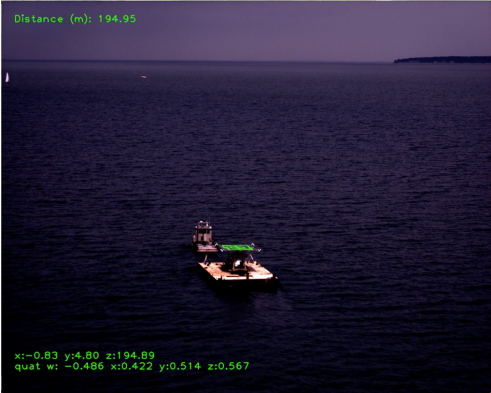
\includegraphics[width=0.6\textwidth]{figs/chp01/chp01_03_CMU_Sea_Landing.pdf}
	\caption{卡内基梅陇大学直升机机载视觉传感器在降落过程中的对降落目标位置和姿态的解算\cite{Grocholsky2016}}
	\label{fig:chp01_03_CMU_Sea_Landing}
\end{figure}

此外,通过机载传感器直接识别机场跑道,也可以视为一种基于合作标识的降落方法。德国宇航中心DLR飞行控制研究所提出了一种利用可见光、红外或雷达图像中的跑道信息估计固定翼飞机的相对位置的方法,并在其研制的ESVS(Enhanced and Synthetic Vision)平台上得到验证\cite{doehler2003robust}。

\subsection{地基传感器引导降落系统} 

用于户外的地基引导系统并不常见,国防科技大学在2011年,提出一种地基引导系统\cite{Ding_master_2011},该系统通过地面摄像机识别无人机上悬挂的红外标记,完成对无人机的引导降落。在目标无人机沿下滑曲线下降至$400\ m$左右的距离时,引导系统开始工作,此时的无人机高度约为$50\ m$;在距离相机$50\ m$距离时,系统的高度分辨率为$0.032\ m$,水平分辨率为$0.26\ m$。该系统的排布如图\ref{fig:chp01_07_ding_master}所示。

\begin{figure}[htb]   
	\centering
	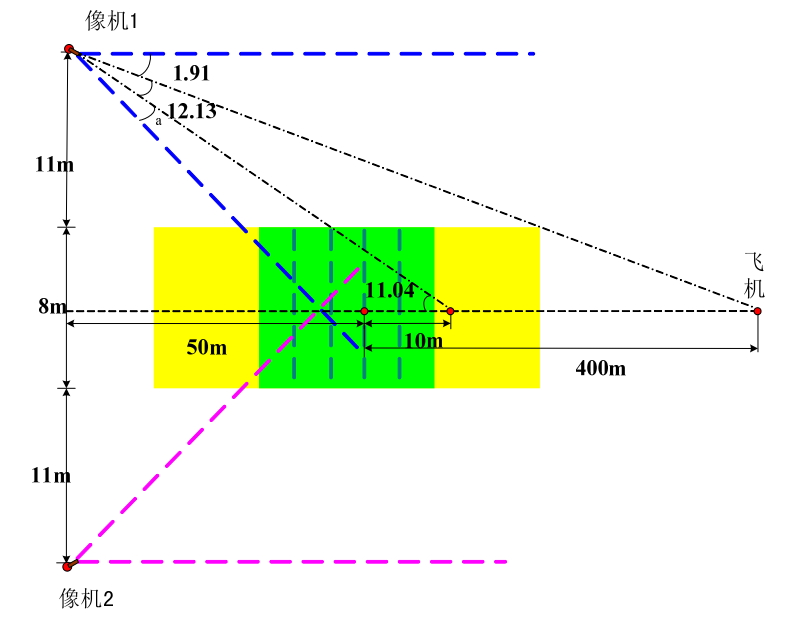
\includegraphics[width=0.6\textwidth]{figs/chp01/chp01_07_ding_master.pdf}
	\caption{地面引导系统排布示意图\cite{Ding_master_2011}}
	\label{fig:chp01_07_ding_master}
\end{figure}

此外,该研究组还提出了采用多台固定焦距摄像机分区域接力测量的方案如图\ref{fig:chp01_08_gui_doctor}所示\cite{gui_doctor_2013}。视觉引导系统由三组摄像机选取不同的焦距,分别观测远场、中场和近场区域,保证相邻两组摄像机视场有一定的重叠区域,并覆盖无人机的下降区域。

\begin{figure}[htb]   
	\centering
	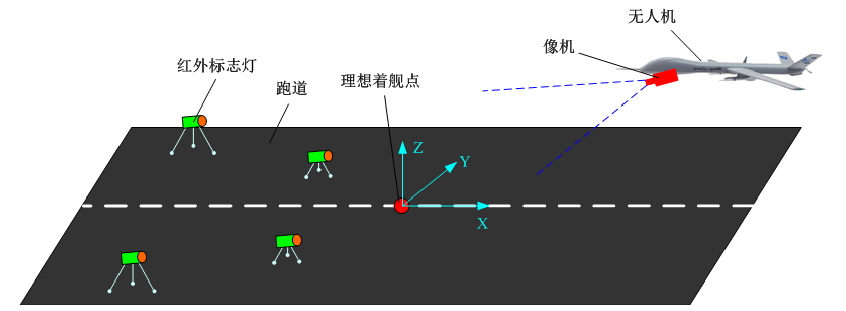
\includegraphics[width=0.6\textwidth]{figs/chp01/chp01_08_gui_doctor.pdf}
	\caption{地基多相机引导系统示意图\cite{gui_doctor_2013}}
	\label{fig:chp01_08_gui_doctor}
\end{figure}

文献\cite{Garcia-Pardo2002}给出了一种基于步进电机和网络摄像头结合的引导设备,可以对微小型无人机进行跟踪,但其视场角受到步进电机的约束。Martinez\cite{Martinez2010}提出了一种三目摄像机系统,如图\ref{fig:chp01_09_three_ground_landing}所示,该系统可以检测无人机的特征点,得到位置信息,但由于构型限制,该系统只适用于旋翼直升机的降落。美国斯坦福大学(Stanford University)\cite{Saripalli2003}使用两个或以上的相机得到了距离$40\ m$外,位置误差约$25\ cm$的视觉系统,但文献中没有具体描述系统的具体结构。日本千叶大学(Chiba University)的研究者\cite{PEBRIANTI2010}使用利用Bumblebee立体视觉传感器,成功将一架四悬翼从$6\ m$的高度引导降落。

\begin{figure}[htb]   
	\centering
	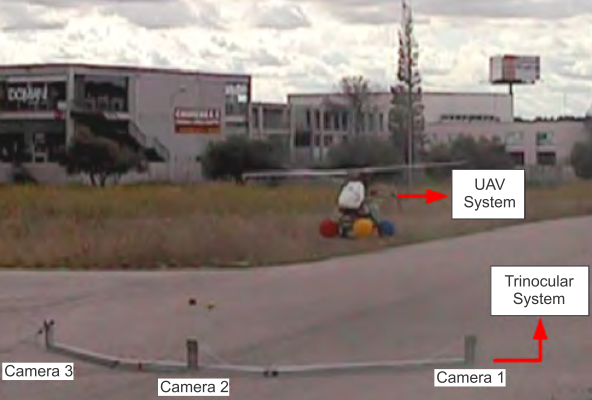
\includegraphics[width=0.7\textwidth]{figs/chp01/chp01_09_three_ground_landing.pdf}
	\caption{地面引导系统排布示意图\cite{Martinez2010}}
	\label{fig:chp01_09_three_ground_landing}
\end{figure}

\section{本文的主要工作、贡献和结构}
本文的主要工作和贡献如下:
(1)提出一种舰基通用的多传感器无人机回收引导系统。该系统主要有两个独立引导单元组成,每个引导单元配备一个二自由度转台和可见光相机、红外相机等传感器。两个独立引导单元的排布可以根据目标无人机的大小和检测距离进行优化配置。本文针对该系统独立分布在跑道两侧的特点,通过对目标位置解算理论推导、误差分析和实验验证,证明了在无人机降落过程中,使用上述两种引导系统的可行性。

(2)提出检测-跟踪-学习相融合的无人机降落过程中实时目标跟踪和位置解算框架。针对引导无人机降落过程中,无人机目标尺度快速变化问题,通过改进基于形态学滤波的图像预处理方法,TLD目标跟踪框架和基于主动轮廓的目标位置修正方法,结合转台运动位置和无人机运动的估计,能够准确解算出无人机在降落过程中相对于舰船的位置信息,满足无人机引导和控制系统的需要。

(3)设计基于非线性模型预测控制(NMPC)和总能量控制(TESC)的无人机着舰控制系统。由于无人机机载设备运算能力的约束,本文设计了内环控制器和外环控制器来实现无人机的自主降落。其中内环控制器主要由PI和PD控制器组成,主要完成对无人机姿态的控制;外环控制器主要由非线性模型预测控制器(NMPC)和总能量控制器(TESC)组成,针对基于Dubins Path生成的降落曲线进行跟踪。

(4)设计并实现无人机舰载着舰系统仿真环境并进行户外实验验证。本文基于机器人操作系统(Robot Operating System,ROS)和Gazebo仿真环境构建了无人机舰载着陆软件在回路仿真系统(SITL)和硬件在回路仿真系统(HIL)。该仿真环境能够满足上述算法的验证需求。通过二自由度转台与多传感器的组合配置,实现在地面机场和水面环境对小型和中型固定翼无人机的引导和自主降落。

本文各个章节的结构图如图\ref{fig:chp01_10_thesis_structure}所示。
\begin{figure}[!h]   
	\centering	
	\includegraphics[width=\textwidth]{figs/chp01/chp01_10_thesis_structure.pdf}
	\caption{本文的组织结构图}
	\label{fig:chp01_10_thesis_structure}
\end{figure}
